\section{iOS}
I dette afsnit beskrives designet af iOS applikationen. I iOS applikationen designes view-klasser, der implementerer view-interfacet defineret i præsentationslaget. Det dominante user interface framework på iOS kaldes UIKit, og det er bygget op omkring en model-view-controller arkitektur. I UIKit har hvert view en tilhørende controller-klasse. I iOS designet tages der højde for dette, ved at bruge controller-klassen som en bro, i mellem Smartpools præsentationslag, og UIKits view-lag. Designet er derfor lavet således, at controller-klasserne på iOS implementerer view-interfacet fra præsentationslaget.

Der findes forskellige basis controller-klasser i UIKit, som kan benyttes. I klasse diagrammet nedenfor, ses iOS designet, med de klasser der implementerer view-interfaces, samt hvilken UIKit controller-klasse de nedarver fra. De views der skal vise en dynamisk liste af data, designes med UITableViewController som superklasse, hvorimod de views der er mere statiske designes med UIViewController som superklasse. 

\begin{figure}
	\centering
	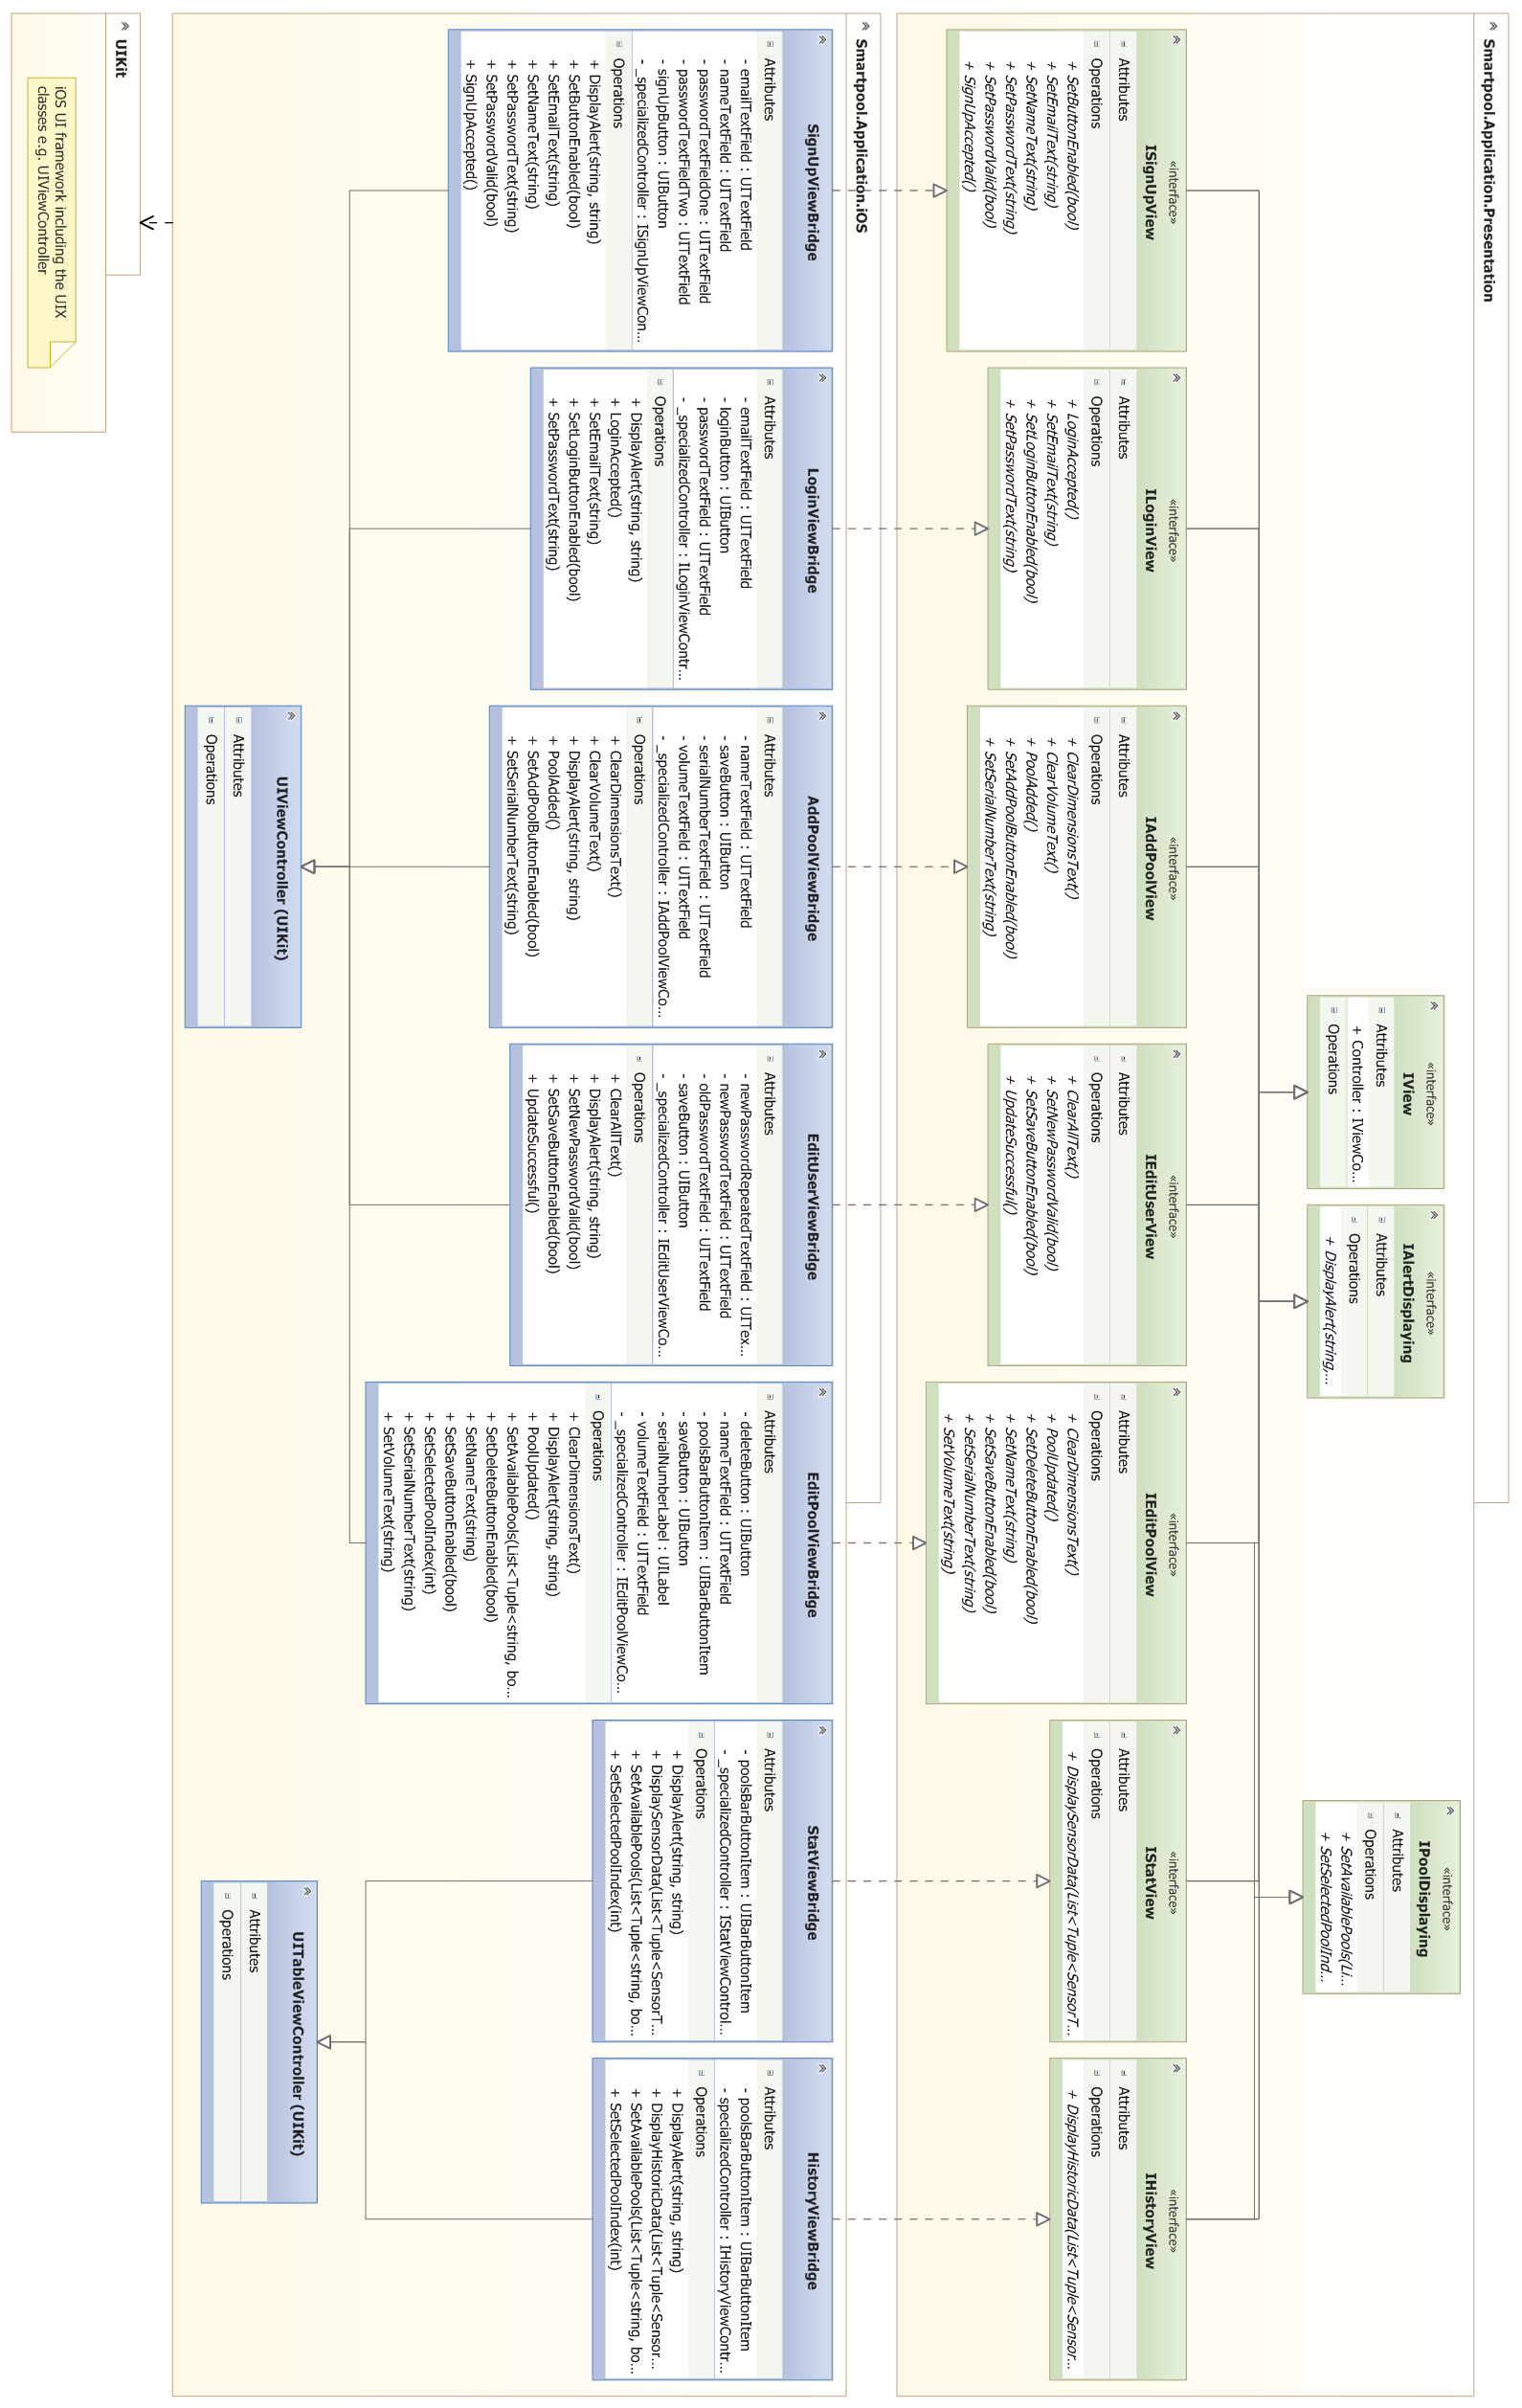
\includegraphics[width=0.9\linewidth]{figs/design/ios_full}
	\caption{iOS applikationens design}
	\label{fig:ios_full}
\end{figure}

Af klassediagrammet fremgår det, at alle iOS klasserne har en "specializedController" property. Dette er en property, der bør typecaste deres nedarvede IViewController property, til den type presenter der passer specifikt til view'et.

\subsection{Klassedesign}
I dette afsnit beskrives designet af de enkelte view-implementerende klasser i Smartpool.Application.iOS. Hver klasse der beskrives i dette afsnit, er en UIKit controller klasse, der implementerer et view-interface defineret i Smartpools præsentationslag.

\subsubsection{SignUpViewBridge}
SignUpViewBridge-klassen implementerer ISignUpView interfacet. Klassen indeholder en række UIKit user interface elementer, som passer sammen med interfacet. Da dette view omhandler brugeroprettelse, er klassen designet til at indeholde en række tekstfelter, og en knap til at fuldende brugeroprettelsen. Denne klasse er designet til at nedarve fra UIKit klassen UIViewController, da de user interface elementer der indgår i designet, forventes at være statiske.

\begin{figure}
	\centering
	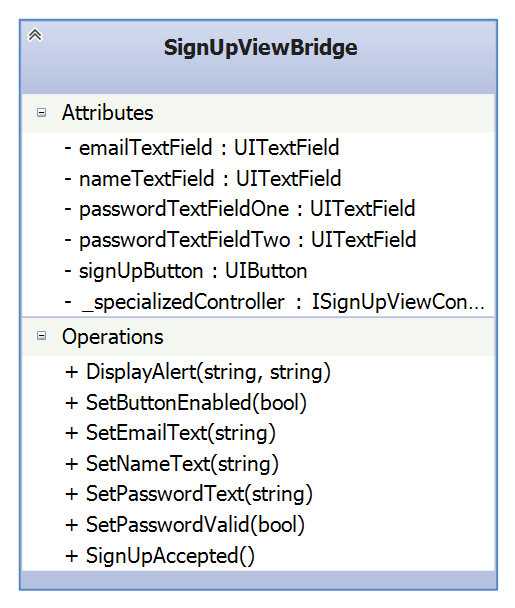
\includegraphics[width=0.3\linewidth]{figs/design/ios_signupviewbridge}
	\caption{SignUpViewBridge}
	\label{fig:ios_signupviewbridge}
\end{figure}

\subsubsection{LoginViewBridge}
LoginViewBridge-klassen implementerer ILoginView interfacet. Da dette view håndtere login, er klassen designet til at indeholde en to tekstfelter, og en knap til at godkende login. Denne klasse er designet til at nedarve fra UIKit klassen UIViewController, da de user interface elementer der indgår i designet, forventes at være statiske.

\begin{figure}
	\centering
	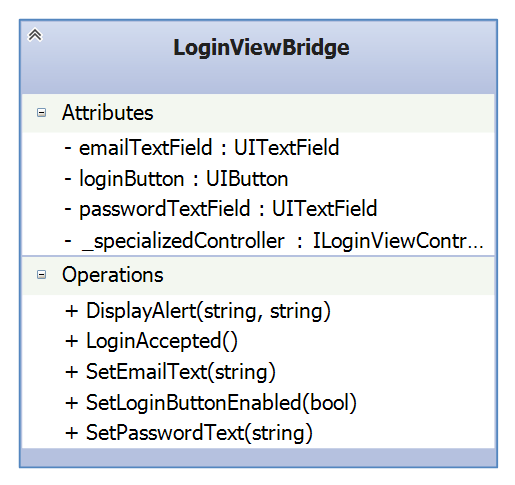
\includegraphics[width=0.3\linewidth]{figs/design/ios_loginviewbridge}
	\caption{LoginViewBridge}
	\label{fig:ios_loginviewbridge}
\end{figure}

\subsubsection{AddPoolViewBridge}
AddPoolViewBridge-klassen implementerer IAddPoolView interfacet. Klassen indeholder en række UIKit user interface elementer, som tekstfelter og en knap, der passer sammen med metoderne i interfacet. Klassen er designet til at nedarve fra UIKit klassen UIViewController, da de user interface elementer der indgår i designet, forventes at være statiske.

\begin{figure}
	\centering
	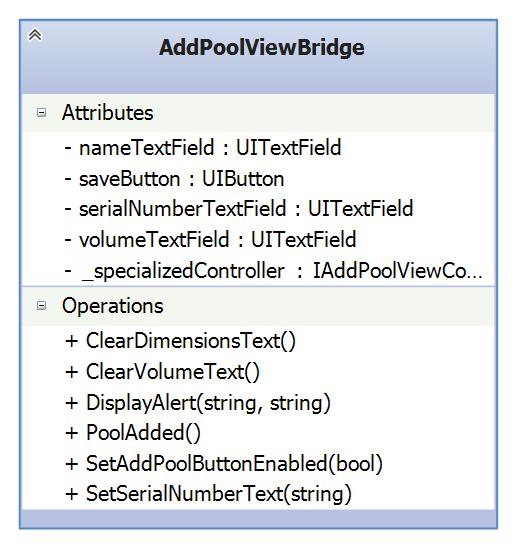
\includegraphics[width=0.3\linewidth]{figs/design/ios_addpoolviewbridge}
	\caption{AddPoolViewBridge}
	\label{fig:ios_addpoolviewbridge}
\end{figure}

\subsubsection{EditUserViewBridge}
Klassen implementerer IEditUserView interfacet. Klassen indeholder en række UIKit user interface elementer, som tekstfelter og en knap, der passer sammen med metoderne i interfacet. Klassen er designet til at nedarve fra UIKit klassen UIViewController, da de user interface elementer der indgår i designet, forventes at være statiske.

\begin{figure}
	\centering
	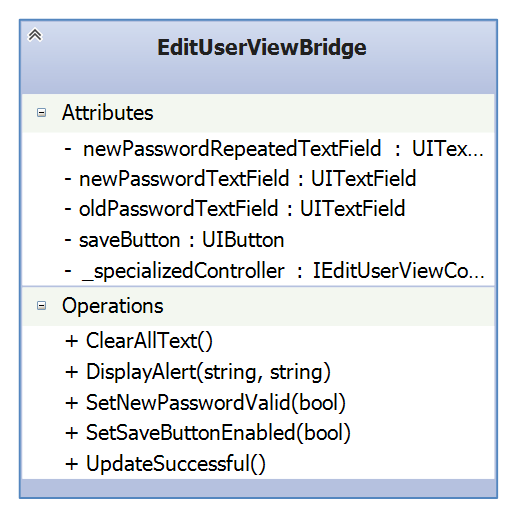
\includegraphics[width=0.3\linewidth]{figs/design/ios_edituserviewbridge}
	\caption{EditUserViewBridge}
	\label{fig:ios_edituserviewbridge}
\end{figure}

\subsubsection{EditPoolViewBridge}
EditPoolViewBridge-klassen implementerer IEditPoolView interfacet. Da dette view håndtere redigering af pools, indeholder klassen tekstfelter, og knap til at foretage ændringer eller slette en pool. Klassen indeholder også en UIBarButtonItem, som type knap, der er tænkt at skulle bruges til skift imellem pools i systemet. Denne knap er tilføjet klassen, da IEditPoolView interfacet implementerer IPoolDisplaying interfacet. Denne klasse er designet til at nedarve fra UIKit klassen UIViewController, da de user interface elementer der indgår i designet, forventes at være statiske.

\begin{figure}
	\centering
	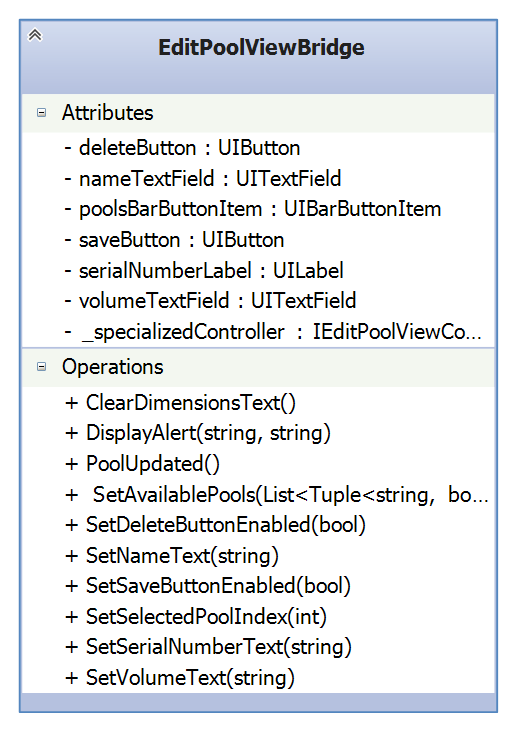
\includegraphics[width=0.3\linewidth]{figs/design/ios_editpoolviewbridge}
	\caption{EditPoolViewBridge}
	\label{fig:ios_editpoolviewbridge}
\end{figure}

\subsubsection{StatViewBridge}
StatViewBridge-klassen implementerer IStatView interfacet. Dette view bør kunne håndtere dynamisk indlæsning og visning af måledata, i følge de user stories der er tilknyttet interfacet. Af denne grund nedarver StatViewBridge fra UITableViewController, der kan opsættes til at præsentere en dynamisk liste. StatViewBridge indeholder en UIBarButtonItem, der kan bruges til at skifte imellem pools i systemet.

\begin{figure}
	\centering
	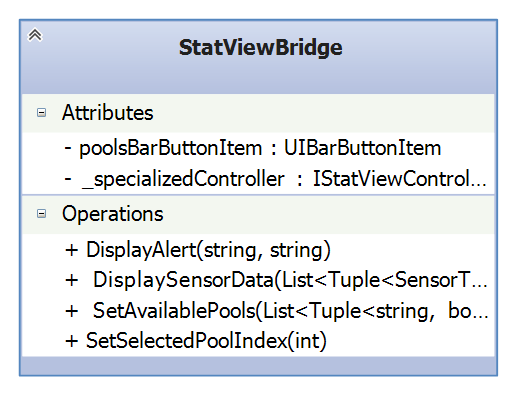
\includegraphics[width=0.3\linewidth]{figs/design/ios_statviewbridge}
	\caption{StatViewBridge}
	\label{fig:ios_statviewbridge}
\end{figure}

\subsubsection{HistoryViewBridge}
HistoryViewBridge-klassen implementerer IHistoryView interfacet. Dette view bør som StatViewBridge kunne håndtere dynamisk indlæsning og visning af måledata. HistoryViewBridge nedarver derfor også fra UITableViewController. Klassen indeholder ligeledes en UIBarButtonItem til skift imellem brugerens pools.

\begin{figure}
	\centering
	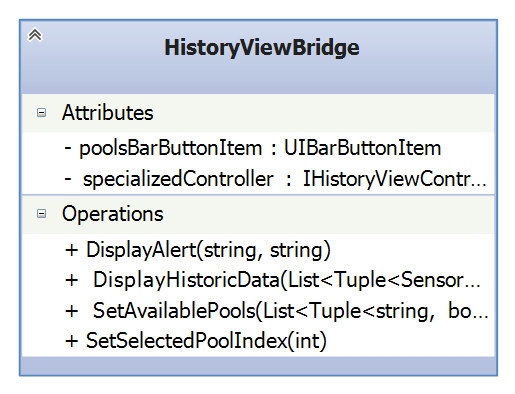
\includegraphics[width=0.3\linewidth]{figs/design/ios_historyviewbridge}
	\caption{HistoryViewBridge}
	\label{fig:ios_historyviewbridge}
\end{figure}